\documentclass[usenames,dvipsnames]{beamer}
\usepackage{colortbl}
\usepackage[utf8]{inputenc}
\usepackage{graphicx}
\usepackage{listings}
\usepackage{fontawesome}

\setlength\extrarowheight{5pt}
\lstdefinestyle{base}{
	language=C++,
	emptylines=1,
	breaklines=true,
	basicstyle=\ttfamily\color{black},
	moredelim=**[is][\bf\color{red}]{@}{@},
}
\lstdefinelanguage{VHDL}{
	morekeywords=[1]{
		library,use,all,entity,is,port,in,out,end,architecture,of,
		begin,and,or,Not,downto,ALL
	},
	morekeywords=[2]{
		STD_LOGIC_VECTOR,std_logic,IEEE,STD_LOGIC_1164,
		NUMERIC_STD,STD_LOGIC_ARITH,STD_LOGIC_UNSIGNED,std_logic_vector,
		std_logic
	},
	morecomment=[l]--
}
\usepackage{xcolor}

\colorlet{keyword}{blue!100!black!80}
\colorlet{STD}{blue!50!red!100!black!80}
\colorlet{comment}{green!80!black!90}
\lstdefinestyle{vhdl}{
	language     = VHDL,
	basicstyle   = \footnotesize \ttfamily,
	keywordstyle = [1]\color{keyword}\bfseries,
	keywordstyle = [2]\color{STD}\bfseries,
	commentstyle = \color{comment}
	breaklines=true,                % sets automatic line breaking
	tabsize=3		                   % sets default tabsize to 2 spaces
}

\usetheme[]{boxes}
\usecolortheme{seagull}
\addtobeamertemplate{navigation symbols}{}{%
	\usebeamerfont{footline}%
	\usebeamercolor[fg]{footline}%
	\hspace{2em}%
	\insertframenumber/\inserttotalframenumber
}
%\usepackage{french}
\title{Modèles et techniques en programmation parallèle hybride et multi-c\oe urs}
\subtitle{Utilisation des accélérateurs de calcul}
\author{Marc Tajchman}\institute{CEA - DEN/DM2S/STMF/LMES}
\date{02/01/2021}
\begin{document}

\begin{frame}
\titlepage
\end{frame}

\large
\begin{frame}
\section{Circuits FPGA}
\frametitle{Circuits FPGA}

Les circuits {\bfseries FPGA} (\underline{\bfseries F}ield-\underline{\bfseries P}rogrammable \underline{\bfseries G}ate \underline{\bfseries A}rray) est constitué d'un ensemble de circuits électroniques (Logic Block dans la figure) connectés entre eux et dont les  paramètres et les connexions (Switch Block, Interconnect) peuvent être changées par l'utilisateur.

\begin{center}
	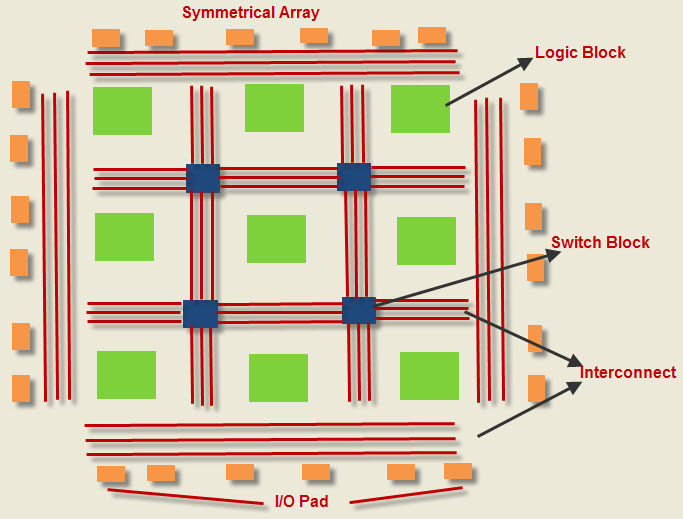
\includegraphics[scale=0.3]{../../Images/FPGA}
	
	Exemple de matrice de circuits FPGA
\end{center}
\end{frame}

\begin{frame}[fragile]
La façon d'utiliser les FPGA dépend de chaque dispositif. 
\vfill
	
En général, l'utilisateur écrit la description du système avec un langage HDL (Hardware Description Language).
\vfill


Exemple:
\begin{minipage}[t]{0.55\textwidth}
\small
\begin{lstlisting}[style=vhdl]
library ieee;
use ieee.std_logic_1164.all;

entity E is
port (
   I1:in std_logic;
   I2:in std_logic;
   O:out std_logic
);
end E;
architecture rtl of E is
signal and_gate: std_logic;
begin
 and_gate <= I1 and I2;
 O <= and_gate;
end rtl;
\end{lstlisting}\end{minipage}
\vfill

\end{frame}

\begin{frame}
On compile ensuite le code en langage HDL qui configure les circuits électroniques et on obtient un système qui peut exécuter seulement l'algorithme contenu dans le programme HDL.

\vfill

L'exécution est très rapide (pas de décodage des instructions) mais pour exécuter autre chose, il faut recompiler un autre code HDL.

\vfill

Utilisé principalement pour des dispositifs très spécialisés (applications embarquées dans les domaines aéronautique, médical,  audio, gps, etc)

\vfill

Catégorie voisine : {\bfseries ASIC} (\underline{\bfseries A}pplication-\underline{\bfseries S}pecific \underline{\bfseries I}ntegrated \underline{\bfseries C}ircuit), encore plus rapides, mais non programmables, les circuits qui exécutent l'algorithme choisi, sont fixés une fois pour toute.
	
\end{frame}

\begin{frame}
\section{Utilisation des GPU}
\frametitle{Utilisation des GPU}

Les GPU (\underline{\bfseries G}raphics \underline{\bfseries P}rocessing \underline{\bfseries U}nits ou cartes graphique) ont été conçus pour faire le plus rapidement possible les calculs nécessaires à l'affichage : affichage pixels couleurs, tracé de formes, projection 3D sur l'écran, etc.
\vfill

\begin{center}
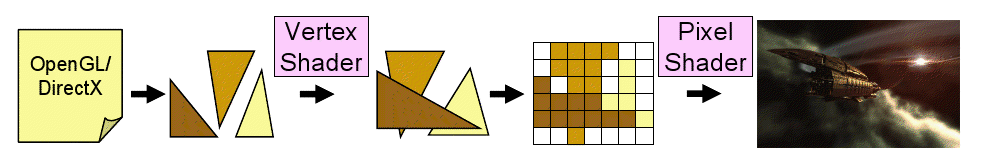
\includegraphics[scale=1.2]{../../Images/GPU_image}
\end{center}

\vfill
Pour programmer les traitements graphiques par les GPU, plusieurs interfaces spécialisées existent (OpenGL, DirectX, Metal, ...).

\vfill

Ces traitements sont souvent très parallélisables et donc les constructeurs de cartes graphiques y incluent beaucoup d'unités de calcul (ou c\oe urs) (plusieurs milliers actuellement).
\vfill

\end{frame}

\begin{frame}
Principales différence entre les CPU et les GPU (situation actuelle) :

\vspace{-0.4cm}
\begin{center}
\begin{tabular}{|l|cl|cl|}
\hline
\rowcolor{Cyan} & & CPU & & GPU \\
\hline
nombre de c\oe urs & \faMehO & $\sim$ 4 à 64 & \faSmileO & $\sim$ 1000 à 10000 \\
\hline
chaque c\oe ur     & \faSmileO & $+$ performant	& \faFrownO &  $-$ performant \\
\hline
jeu d'instructions & \faSmileO & plus général   & \faMehO &  spécialisé calcul \\
\hline
bande passante     & \faFrownO & $-$ importante & \faSmileO & $+$ importante \\
\hline
latence            & \faSmileO & $+$ petite & \faFrownO & $+$ grande \\
\hline
\end{tabular}
\end{center}

Ici, latence, bande passante : durée initialisation et quantité échangée par seconde entre la mémoire et le processeur.

\vfill
\end{frame}

\begin{frame}

\vfill
La puissance de calcul (nombre de c\oe urs $\times$ performance d'un c\oe ur) des GPU dépassent celle des CPU : les c\oe urs GPU sont moins puissants que les c\oe urs CPU mais (beaucoup) plus nombreux.

\begin{center}
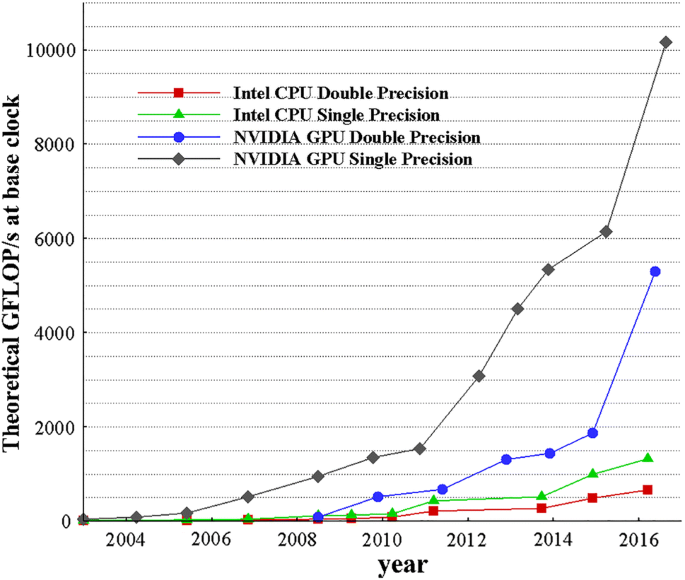
\includegraphics[scale=0.3]{../../Images/Perf_CPU_GPU}
\end{center}
\vfill
\end{frame}

\begin{frame}
	Pourquoi une telle différence ?
	\vfill
	\begin{itemize}
		\item \textcolor{blue}{Les CPU exécutent tous les traitements, parallèles ou non}
		
	\vfill
		\begin{quote}
		Par conception, les CPU sont optimisés pour des calculs séquentiels : beaucoup de mémoire cache, plusieurs additionneurs/multiplicateurs, prédiction de branches, exécution d'instructions ``dans le désordre'' (out-of-order)
		 \end{quote}
	 
	 \vfill
		\item \textcolor{blue}{Les GPU supposent que le degré de parallélisme est élevé}
		
	\vfill
		\begin{quote}
        Par conception, les GPU maximisent la bande passante utilisable par beaucoup de threads, moins de mémoire cache (latence compensée par le multithreads massif), circuits de contrôle partagés entre les threads
   		\end{quote}
	
		
	\end{itemize}
\end{frame}

\begin{frame}
Structure interne comparée (schématique):

\begin{itemize}
	\item ALU : c\oe ur
	\item Control : contrôleur mémoire
	\item Cache : mémoire cache
	\item DRAM : mémoire de travail
\end{itemize}

\vfill
\hbox{\begin{minipage}[c]{0.5\textwidth}
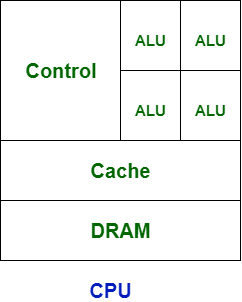
\includegraphics[scale=0.4]{../../Images/CPU}
\end{minipage}
\begin{minipage}[c]{0.5\textwidth}
	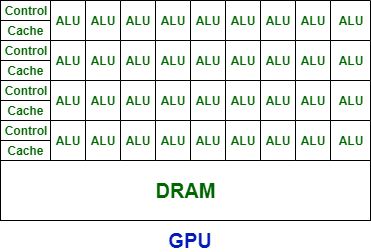
\includegraphics[scale=0.4]{../../Images/GPU}
\end{minipage}
}
\end{frame}

\begin{frame}
Sur une seule machine, pour :
\begin{tabular}{ll}
calculs séquentiels ou faiblement // :& utiliser le CPU \\
calculs fortement // :& utiliser le GPU
\end{tabular}

\vfill

A adapter à chaque cas !!

\vfill

Les résultats ne seront pas toujours exactement les mêmes sur CPU et sur GPU:
\begin{itemize}
\item Jusque $\sim$ 2000, les GPU (Nvidia) calculaient seulement en simple précision (32 bits) : pas besoin de 15 décimales pour calculer la couleur de pixels
\item Depuis, on a du 64 bits (double précision) sur GPU, {\bfseries mais} pas toujours les mêmes précisions entre le GPU et le CPU pour les additions/multiplications/divisions/..., les modes d'arrondi ne sont pas toujours identiques
\end{itemize}

\end{frame}

\begin{frame}
	Jusque 2000, la seule façon de programmer les GPU est l'utilisation de OpenGL, DirectX, etc.
	
	A partir de 2000, apparaissent les modèles de programmation Cuda ()
\end{frame}

\begin{frame}
\end{frame}

\begin{frame}
\end{frame}

\end{document}
